\documentclass[11pt]{scrartcl}
\usepackage[T1]{fontenc}
\usepackage[utf8]{inputenc}

\title{Computer Systems Week 3 Lab}
\author{Daniel Coady (102084174)}
\date{21/08/2019}

\usepackage{graphicx}

\begin{document}

\maketitle

% 4 bit register
\begin{center}
    \begin{tabular}{c|c c}
        \multicolumn{3}{c}{Big Endian 4 Bit Register} \\[1em]
        \hline
        Qx & input & output \\
        \hline
        0 & 0000 & 0000 \\
        1 & 0001 & 0001 \\
        2 & 0010 & 0010 \\
        3 & 0011 & 0011 \\
        4 & 0100 & 0100 \\
        5 & 0101 & 0101 \\
        6 & 0110 & 0110 \\
        7 & 0111 & 0111 \\
        8 & 1000 & 1000 \\
        9 & 1001 & 1001 \\
        A & 1010 & 1010 \\
        B & 1011 & 1011 \\
        C & 1100 & 1100 \\
        D & 1101 & 1101 \\
        E & 1110 & 1110 \\
        F & 1111 & 1111 \\
    \end{tabular}

    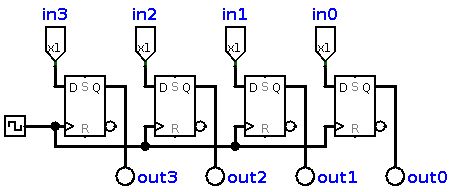
\includegraphics[scale=0.5]{images/bigendian4bitregister.png}
\end{center}

Hardware counters are useful for things like progress displays, especially
on simpler pieces of hardware that might not have or need software implementations
to operate.

A ripple counter works similar to how the name implies. Every JK flip flop
in the counter has both the J and K inputs on so that it works as a T flip flop.
The thing that makes this work then is that clock input, since each JK flip flop
has it's clock input connected to the previous one's Q output. Because of this
each subsequent flip flop will only be able to toggle it's input once the previous
flip flop's Q output is on, "rippling" the counting down the chain of flip flops.

\begin{figure}[h]
    \centering
    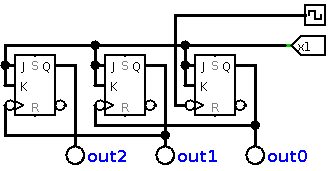
\includegraphics[scale=0.5]{images/bigendian3bitripplecounter.png}
    \caption{Big endian 3 bit ripple counter}
\end{figure}

\begin{figure}[h]
    \centering
    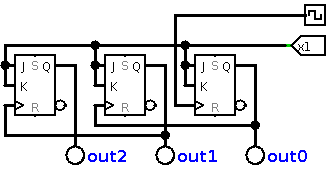
\includegraphics[scale=0.5]{images/bigendian3bitreverseripplecounter.png}
    \caption{Big endian 3 bit reverse ripple counter}
\end{figure}

\begin{figure}[h]
    \centering
    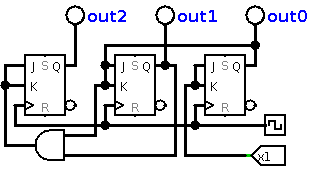
\includegraphics[scale=0.5]{images/bigendian3bitcommonclockcounter.png}
    \caption{Big endian 3 bit common clock counter}
\end{figure}

\pagebreak

\begin{figure}[h]
    \centering
    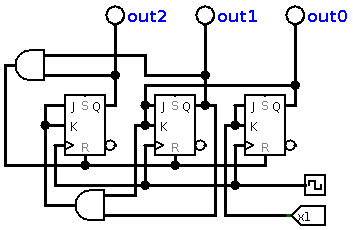
\includegraphics[scale=0.5]{images/bigendian3bitcommonclockcountermod6.png}
    \caption{Big endian 3 bit common clock counter MOD 6}
\end{figure}

\begin{figure}[h]
    \centering
    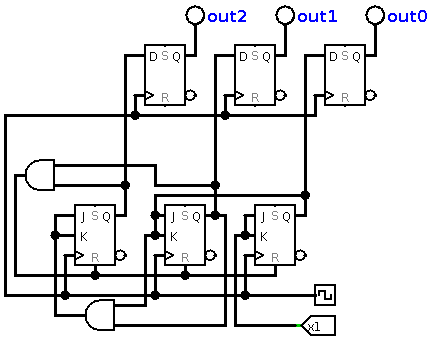
\includegraphics[scale=0.5]{images/bigendian3bitcommonclockcountermod6withregister.png}
    \caption{Big endian 3 bit common clock counter MOD 6 with register}
\end{figure}

Using a register to handle illegal states is very important because while we are
just simulating things within a program where timing between things is very consistent
and easy to predict, if an illegal state slips by in an actual physical circuit then
you may run into issues with that state in a later part of the circuit that it feeds into,
causing unpredictable behaviour.

\pagebreak

\begin{figure}[h]
    \centering
    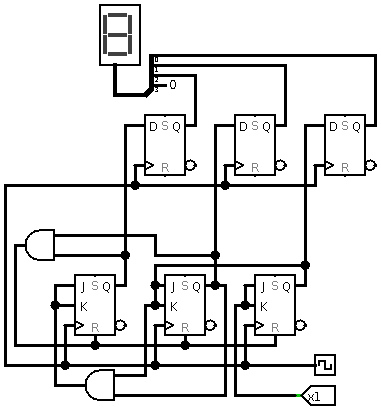
\includegraphics[scale=0.5]{images/bigendian3bitcommonclockcountermod6withregisterhexdisplay.png}
    \caption{Big endian 3 bit common clock counter MOD 6 with register and hex display}
\end{figure}

\end{document}
